% ------------------------------------------------------------

\begin{frame}

\frametitle{\TeX: а что это?}

\begin{itemize}[<+->]
    \item Система вёрстки статей, дипломов, презентаций, \dots
    \item Придумана и имплементирована Дональдом Кнутом
    \item Первый релиз в 1978
    \item Де-факто стандарт (как минимум в computer science)
    \item WYSIWYM (What You See Is What You Mean) 
    в противопоставление WYSIWYG (What You See Is What You Get),
    что как раз происходит в MS Word
\end{itemize}

\end{frame}

% ------------------------------------------------------------

\begin{frame}

\frametitle{\TeX: внешний вид}

{

\captionsetup[subfloat]{labelformat=empty}

\begin{figure}[c]
  \centering
  \subfloat[Текст с выкладками]
  {\raisebox{30pt}{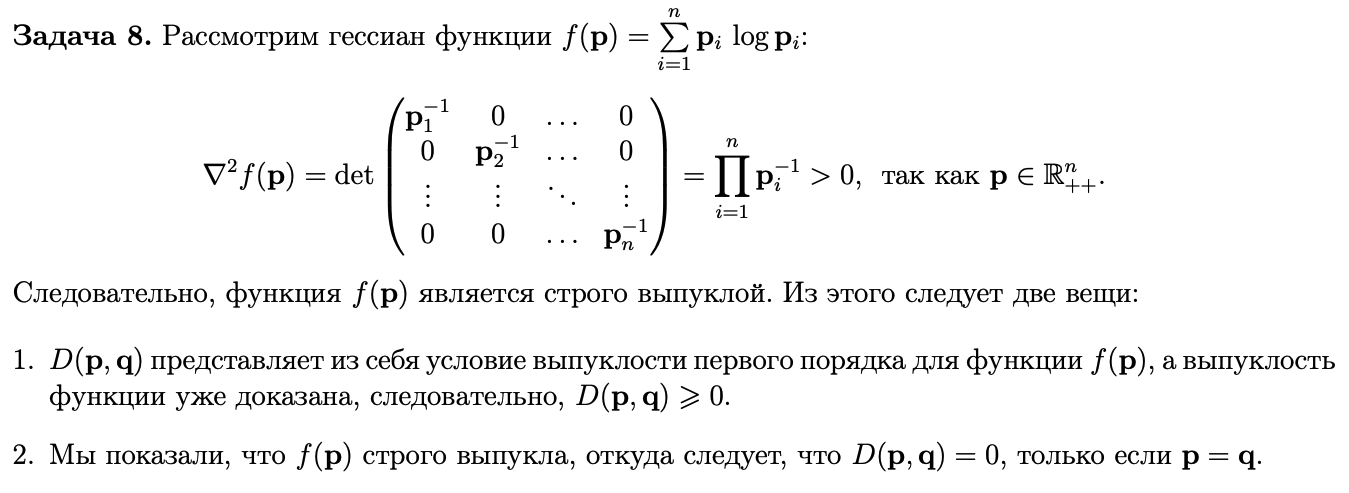
\includegraphics[width=0.48\textwidth]{images/tex-example-more-text.png}}}
  \quad
  \subfloat[Выкладки с текстом]
  {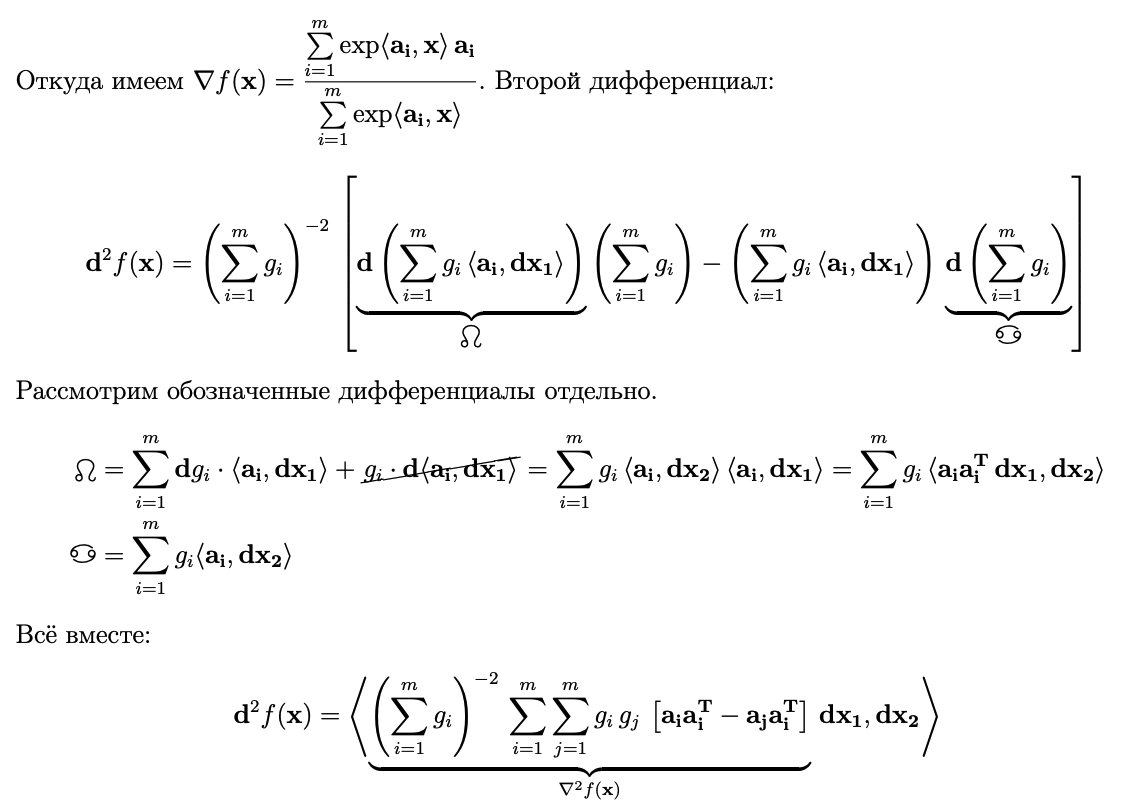
\includegraphics[width=0.48\textwidth]{images/tex-example-more-formulae.png}}
\end{figure}

}

\end{frame}
